%% abtex2-modelo-include-comandos.tex, v-1.4 laurocesar
%% Copyright 2012-2013 by abnTeX2 group at http://abntex2.googlecode.com/ 
%%
%% This work may be distributed and/or modified under the
%% conditions of the LaTeX Project Public License, either version 1.3
%% of this license or (at your option) any later version.
%% The latest version of this license is in
%%   http://www.latex-project.org/lppl.txt
%% and version 1.3 or later is part of all distributions of LaTeX
%% version 2005/12/01 or later.
%%
%% This work has the LPPL maintenance status `maintained'.
%% 
%% The Current Maintainer of this work is the abnTeX2 team, led
%% by Lauro César Araujo. Further information are available on 
%% http://abntex2.googlecode.com/
%%
%% This work consists of the files abntex2-modelo-include-comandos.tex
%%

% ---
% Este capítulo, utilizado por diferentes exemplos do abnTeX2, ilustra o uso de
% comandos do abnTeX2 e de LaTeX.
% ---
 
\chapter{Questionário de pesquisa}\label{questionario_de_pesquisa}

Neste apêndice serão apresentados os formulários de pesquisa utilizados para coletar informações dos participantes, destacando a diferenciação entre os dois questionários aplicados. A separação dos participantes em grupos de profissionais e estudantes foi uma etapa fundamental deste estudo, pois, embora os questionários sejam estruturalmente semelhantes, eles diferem na primeira parte, onde foram apresentadas perguntas demográficas e de conhecimento aos participantes.

Os dois questionários empregados neste estudo foram desenhados para coletar dados sobre as percepções dos participantes em relação às telas de \ac{UI} e \ac{UX}. Ambos os questionários compartilharam uma série de perguntas idênticas, com o propósito de avaliar as telas de login, cadastro, tela principal e tela de conteúdo. A distinção crítica entre os questionários ocorreu na primeira parte, na qual as perguntas demográficas e de conhecimento foram apresentadas aos participantes.

\newpage
\section{Primeira Parte}

Neste estágio específico do questionário, ocorre a distinção de questionamentos, como mencionado anteriormente, entre os dois grupos em análise. As Figuras \ref{AP_P01}, \ref{AP_PPr}, \ref{AP_PEs} e \ref{AP_P02} referem-se a parte inicial dos questionários, com questões para qualificação dos respondentes, sendo que as Figuras \ref{AP_P01} e \ref{AP_P02} referem-se às questões aplicadas à ambos os participantes, a \autoref{AP_PPr} refere-se apenas à profissionais e \autoref{AP_PEs} refere-se apenas à estudantes.

\begin{figure}[!h]
	\begin{center}
	    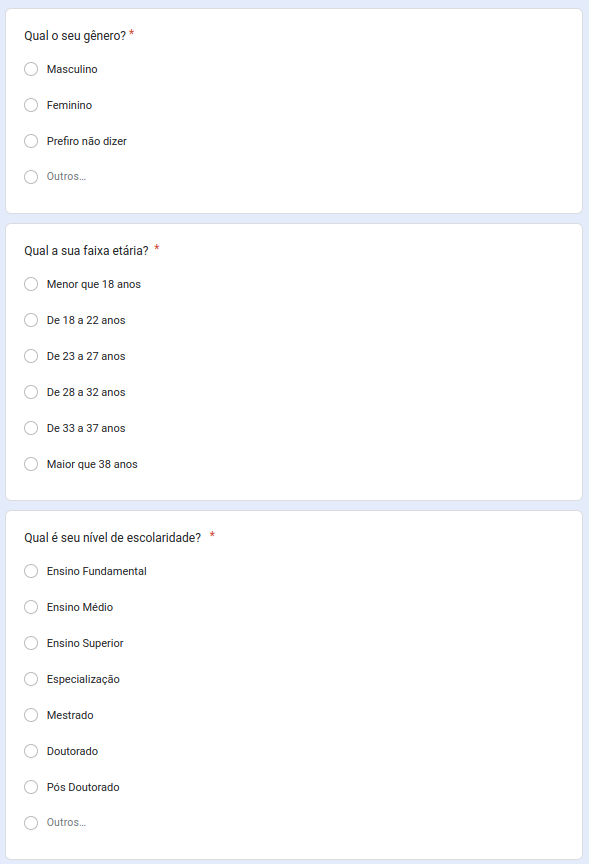
\includegraphics[scale=0.8]{figs/Form/01.png}
	\end{center}
	\caption{\label{AP_P01}Formulário de pesquisa com ambos participantes - Parte 1}
\end{figure}

\newpage

\begin{figure}[!h]
	\begin{center}
	    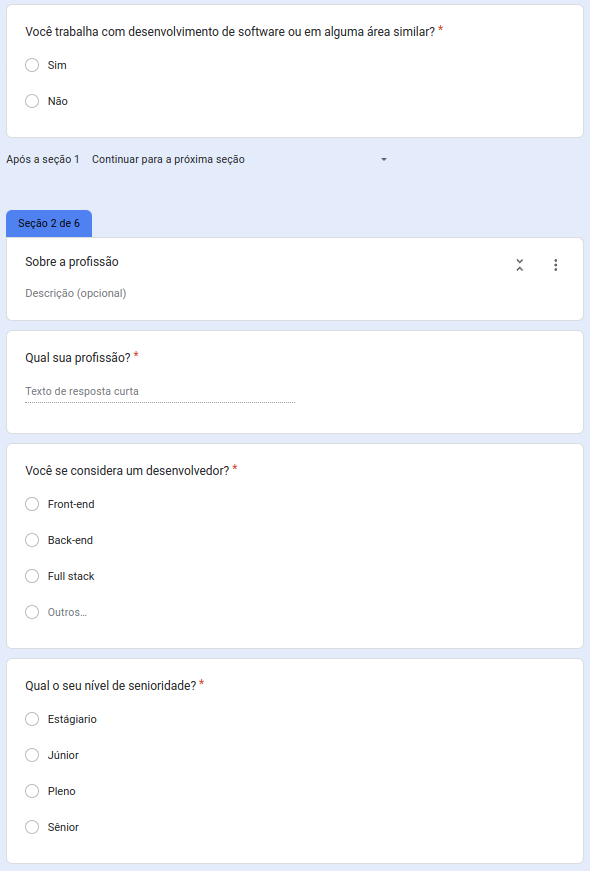
\includegraphics[scale=0.6]{figs/Form/02.png}
	\end{center}
	\caption{\label{AP_PPr}Formulário de pesquisa apenas profissionais - Parte Profissionais}
\end{figure}

\newpage

\begin{figure}[!h]
	\begin{center}
	    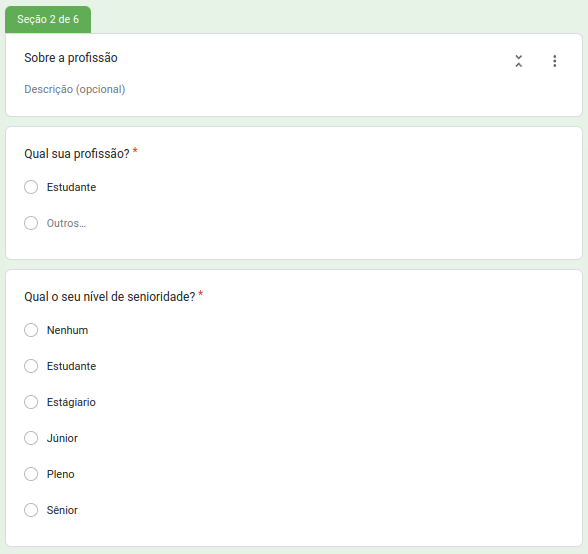
\includegraphics[scale=0.6]{figs/Form/03.png}
	\end{center}
	\caption{\label{AP_PEs}Formulário de pesquisa apenas estudantes - Parte Estudantes}
\end{figure}

\begin{figure}[!h]
	\begin{center}
	    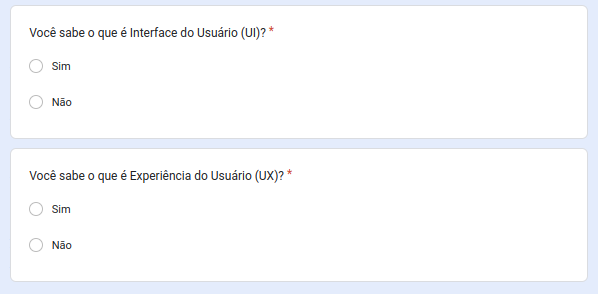
\includegraphics[scale=0.6]{figs/Form/04.png}
	\end{center}
	\caption{\label{AP_P02}Formulário de pesquisa com ambos participantes - Parte 2}
\end{figure}

\newpage

\section{Questionário}

Nas subseções a seguir todas as perguntas presentes nas Figuras são destinadas a ambos os grupos.

\subsection{Tela de Login}

As Figuras \ref{AP_LP01}, \ref{AP_LP02}, \ref{AP_LP03}, \ref{AP_LP04} referem-se à tela de login.

\begin{figure}[!h]
	\begin{center}
	    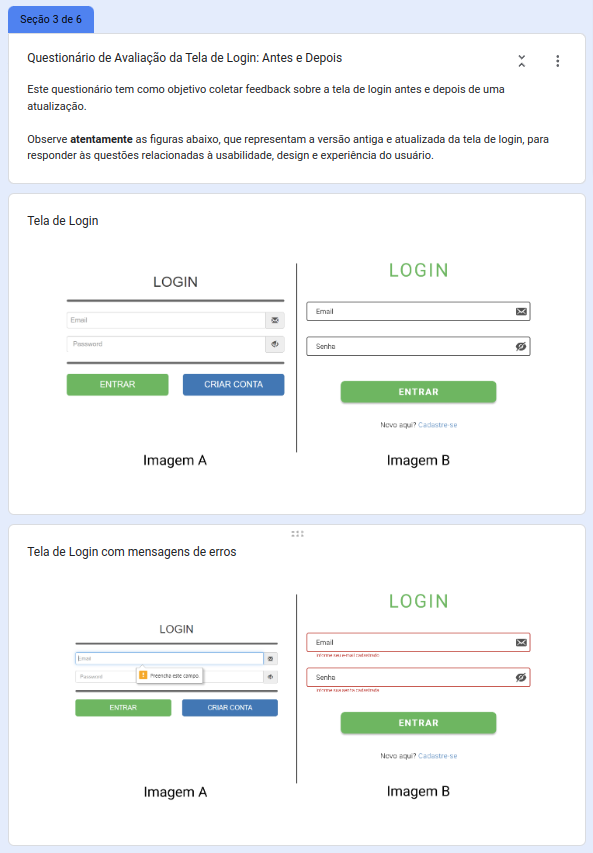
\includegraphics[scale=0.6]{figs/Form/05.png}
	\end{center}
	\caption{\label{AP_LP01}Formulário de pesquisa, Login - Parte 1}
\end{figure}

\newpage

\begin{figure}[!h]
	\begin{center}
	    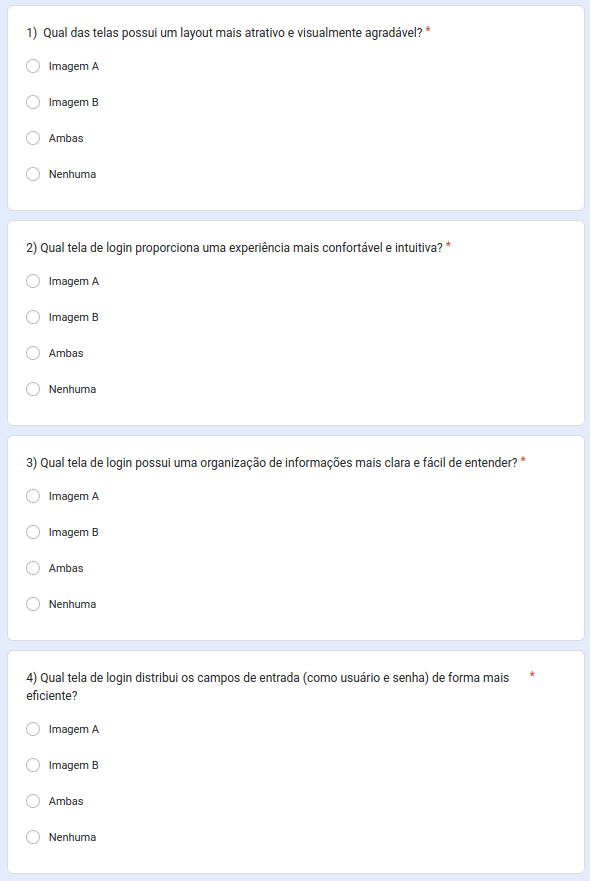
\includegraphics[scale=0.6]{figs/Form/06.png}
	\end{center}
	\caption{\label{AP_LP02}Formulário de pesquisa, Login - Parte 2}
\end{figure}

\newpage

\begin{figure}[!h]
	\begin{center}
	    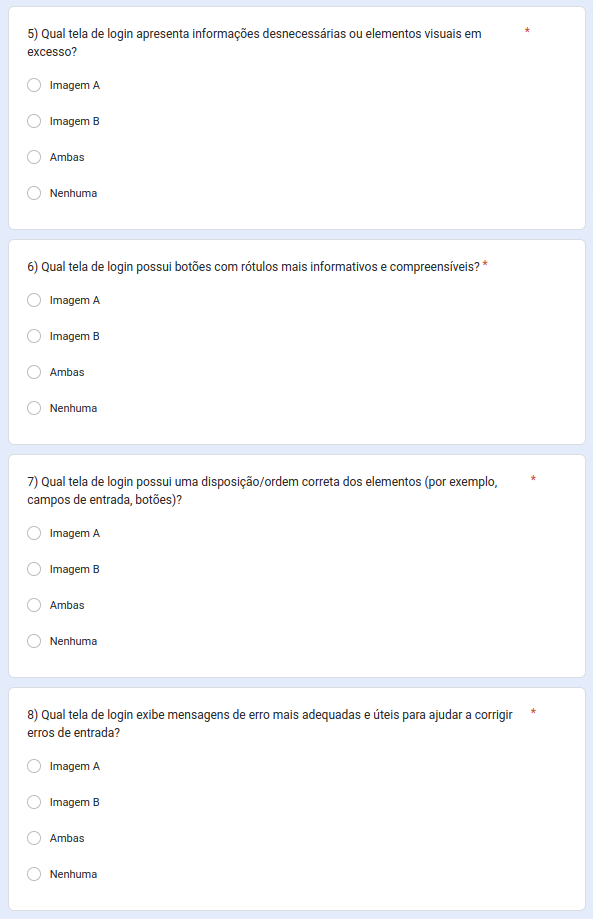
\includegraphics[scale=0.6]{figs/Form/07.png}
	\end{center}
	\caption{\label{AP_LP03}Formulário de pesquisa, Login - Parte 3}
\end{figure}

\newpage

\begin{figure}[!h]
	\begin{center}
	    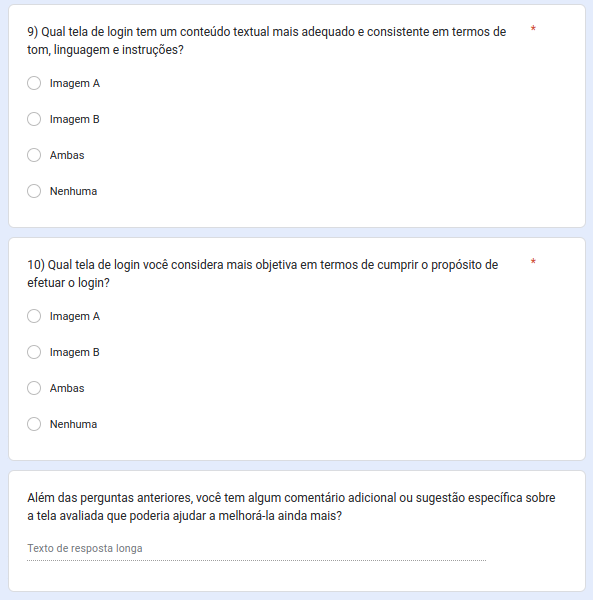
\includegraphics[scale=0.6]{figs/Form/08.png}
	\end{center}
	\caption{\label{AP_LP04}Formulário de pesquisa, Login - Parte 4}
\end{figure}

\newpage

\subsection{Tela de Cadastro}

As Figuras \ref{AP_CP01}, \ref{AP_CP02}, \ref{AP_CP03}, \ref{AP_CP04} referem-se à tela de cadastro.

\begin{figure}[!h]
	\begin{center}
	    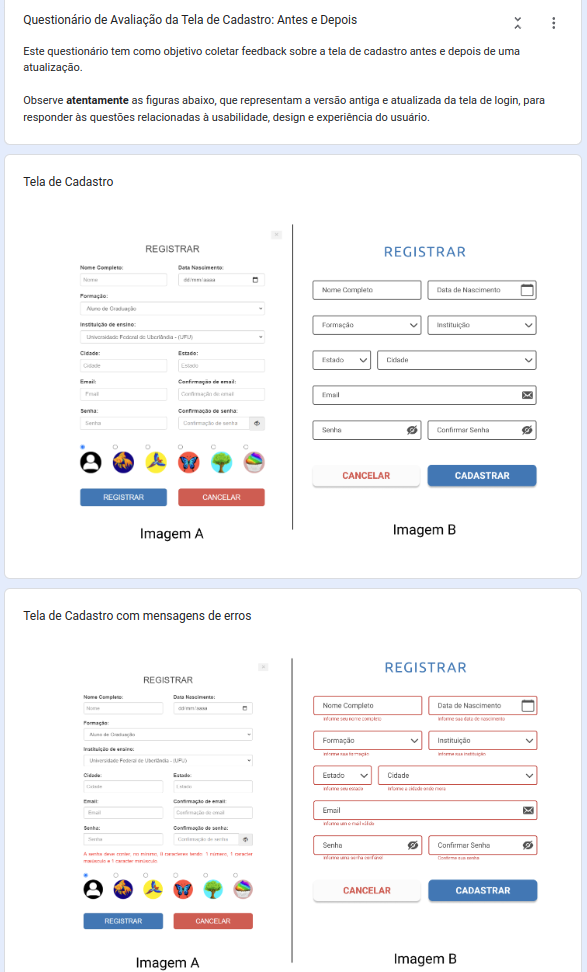
\includegraphics[scale=0.6]{figs/Form/09.png}
	\end{center}
	\caption{\label{AP_CP01}Formulário de pesquisa, Cadastro - Parte 1}
\end{figure}

\newpage

\begin{figure}[!h]
	\begin{center}
	    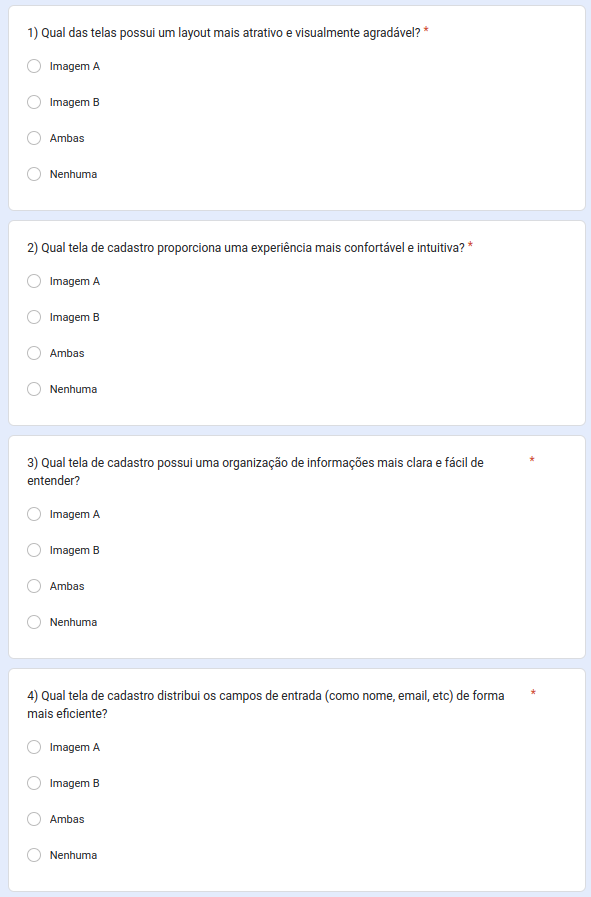
\includegraphics[scale=0.6]{figs/Form/10.png}
	\end{center}
	\caption{\label{AP_CP02}Formulário de pesquisa, Cadastro - Parte 2}
\end{figure}

\newpage

\begin{figure}[!h]
	\begin{center}
	    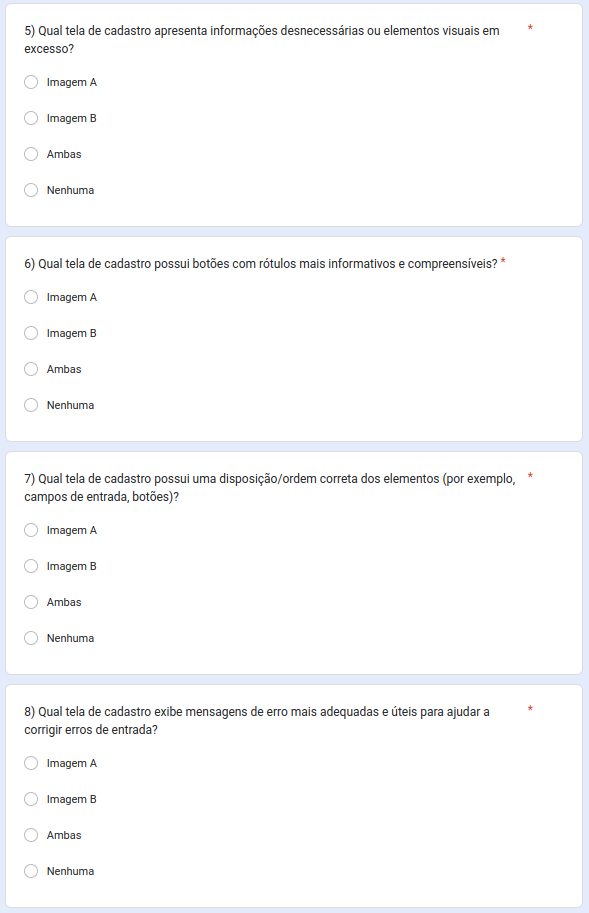
\includegraphics[scale=0.6]{figs/Form/11.png}
	\end{center}
	\caption{\label{AP_CP03}Formulário de pesquisa, Cadastro - Parte 3}
\end{figure}

\newpage

\begin{figure}[!h]
	\begin{center}
	    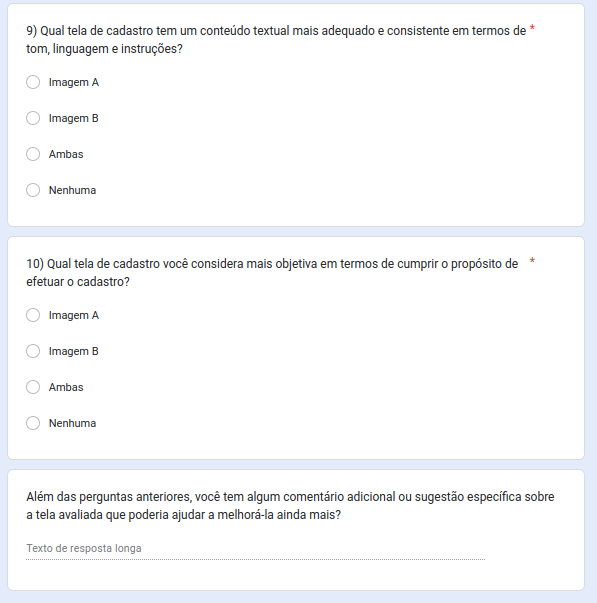
\includegraphics[scale=0.6]{figs/Form/12.png}
	\end{center}
	\caption{\label{AP_CP04}Formulário de pesquisa, Cadastro - Parte 4}
\end{figure}

\newpage

\subsection{Tela de Principal}

As Figuras \ref{AP_PP01}, \ref{AP_PP02}, \ref{AP_PP03}, \ref{AP_PP04}, \ref{AP_PP05}, \ref{AP_PP06} referem-se à tela de principal.

\begin{figure}[!h]
	\begin{center}
	    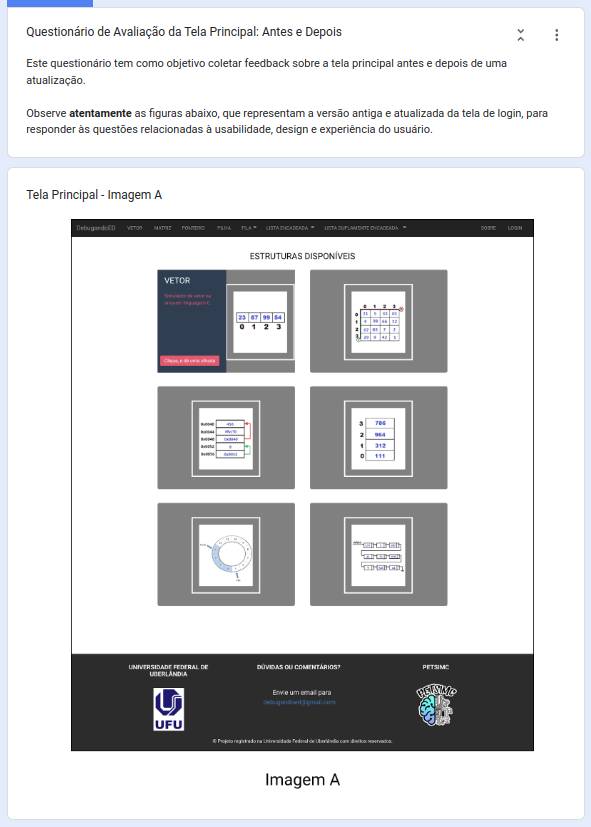
\includegraphics[scale=0.6]{figs/Form/13.png}
	\end{center}
	\caption{\label{AP_PP01}Formulário de pesquisa, Principal - Parte 1}
\end{figure}

\newpage

\begin{figure}[!h]
	\begin{center}
	    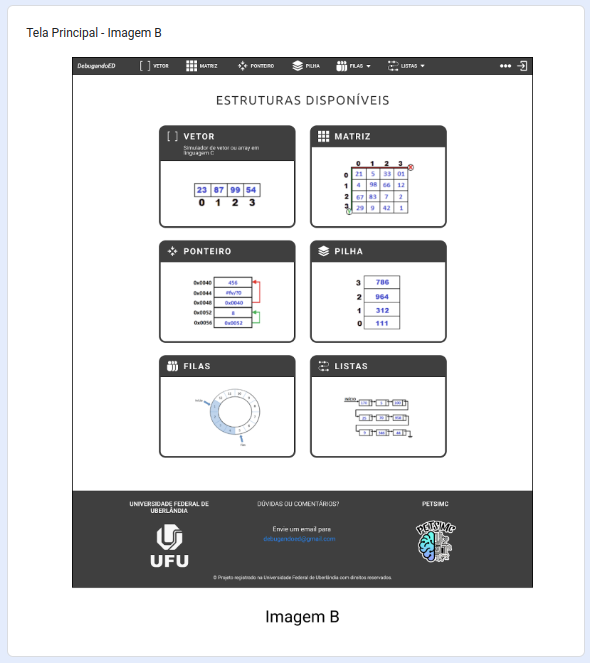
\includegraphics[scale=0.6]{figs/Form/14.png}
	\end{center}
	\caption{\label{AP_PP02}Formulário de pesquisa, Principal - Parte 2}
\end{figure}

\newpage

\begin{figure}[!h]
	\begin{center}
	    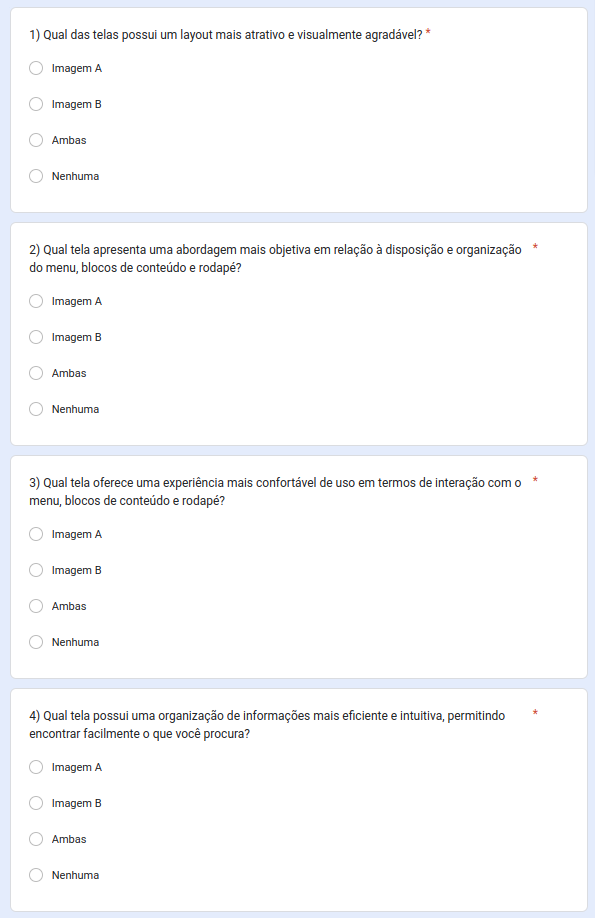
\includegraphics[scale=0.6]{figs/Form/15.png}
	\end{center}
	\caption{\label{AP_PP03}Formulário de pesquisa, Principal - Parte 3}
\end{figure}

\newpage

\begin{figure}[!h]
	\begin{center}
	    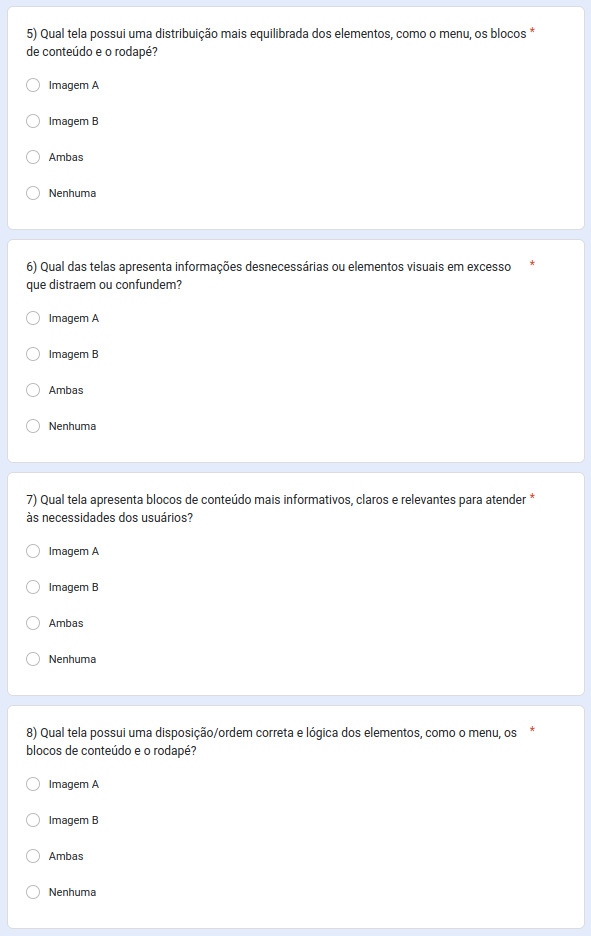
\includegraphics[scale=0.6]{figs/Form/16.png}
	\end{center}
	\caption{\label{AP_PP04}Formulário de pesquisa, Principal - Parte 4}
\end{figure}

\newpage

\begin{figure}[!h]
	\begin{center}
	    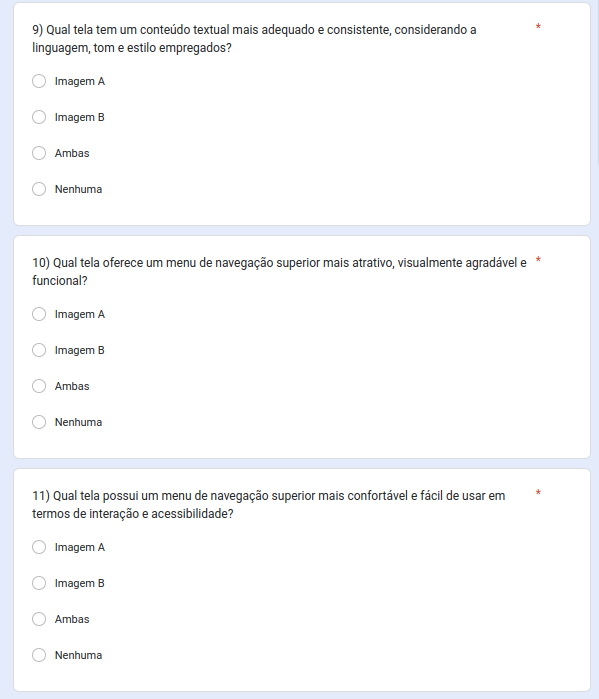
\includegraphics[scale=0.6]{figs/Form/17.png}
	\end{center}
	\caption{\label{AP_PP05}Formulário de pesquisa, Principal - Parte 5}
\end{figure}

\newpage

\begin{figure}[!h]
	\begin{center}
	    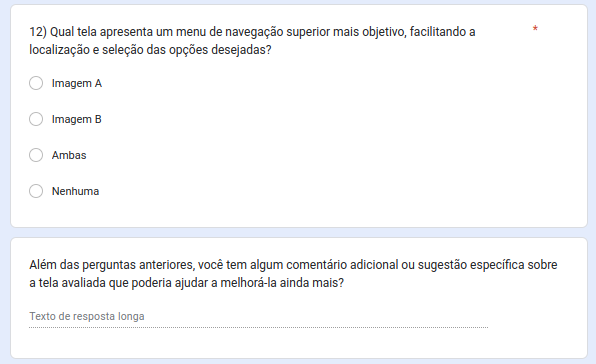
\includegraphics[scale=0.6]{figs/Form/18.png}
	\end{center}
	\caption{\label{AP_PP06}Formulário de pesquisa, Principal - Parte 6}
\end{figure}

\newpage

\subsection{Tela de Ponteiro}

As Figuras \ref{AP_PonP01}, \ref{AP_PonP02}, \ref{AP_PonP03}, \ref{AP_PonP04} referem-se à tela de ponteiro.

\begin{figure}[!h]
	\begin{center}
	    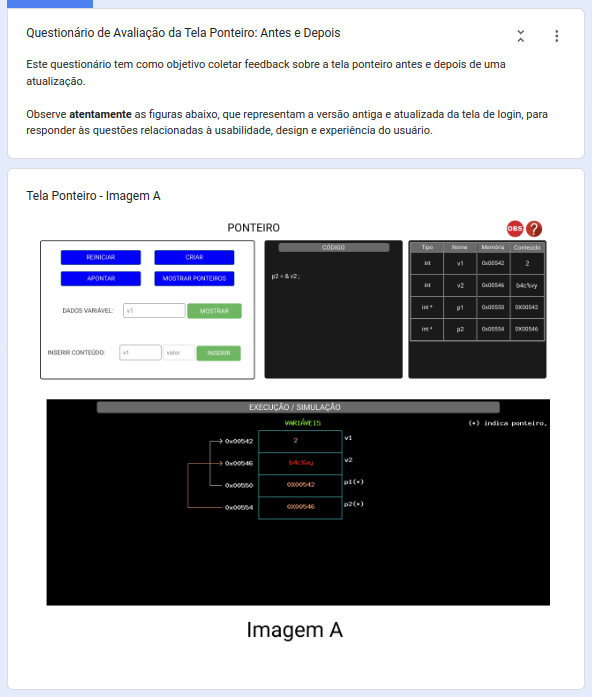
\includegraphics[scale=0.6]{figs/Form/19.png}
	\end{center}
	\caption{\label{AP_PonP01}Formulário de pesquisa, Ponteiro - Parte 1}
\end{figure}

\newpage

\begin{figure}[!h]
	\begin{center}
	    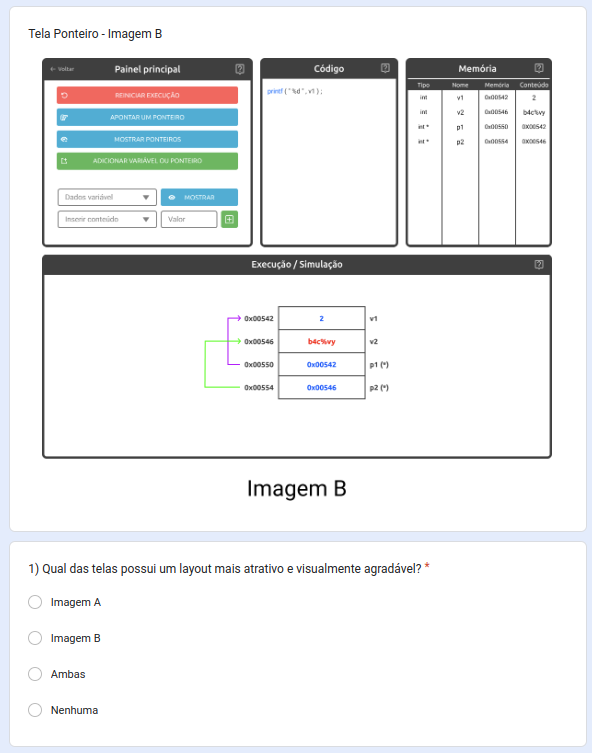
\includegraphics[scale=0.6]{figs/Form/20.png}
	\end{center}
	\caption{\label{AP_PonP02}Formulário de pesquisa, Ponteiro - Parte 2}
\end{figure}

\newpage

\begin{figure}[!h]
	\begin{center}
	    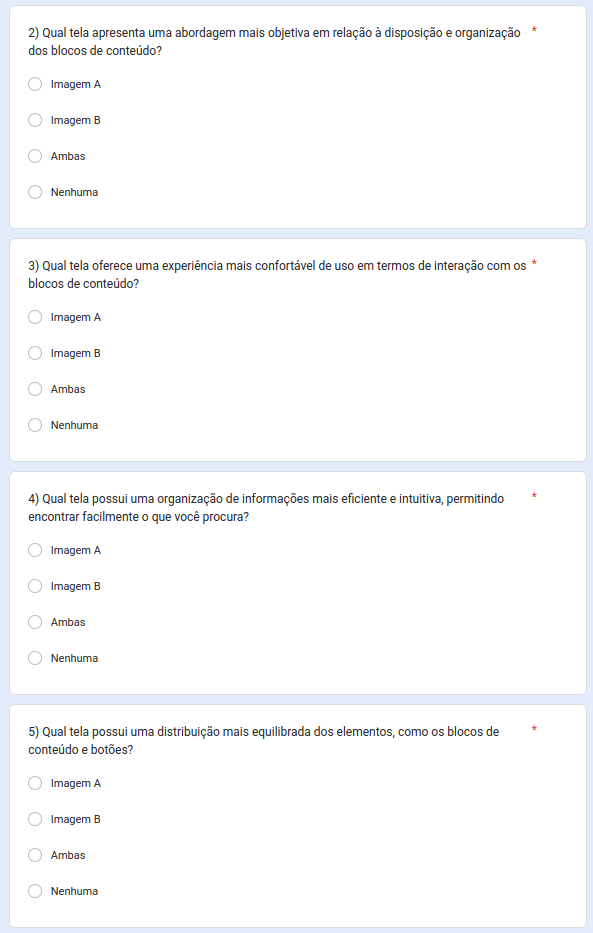
\includegraphics[scale=0.6]{figs/Form/21.png}
	\end{center}
	\caption{\label{AP_PonP03}Formulário de pesquisa, Ponteiro - Parte 3}
\end{figure}

\newpage

\begin{figure}[!h]
	\begin{center}
	    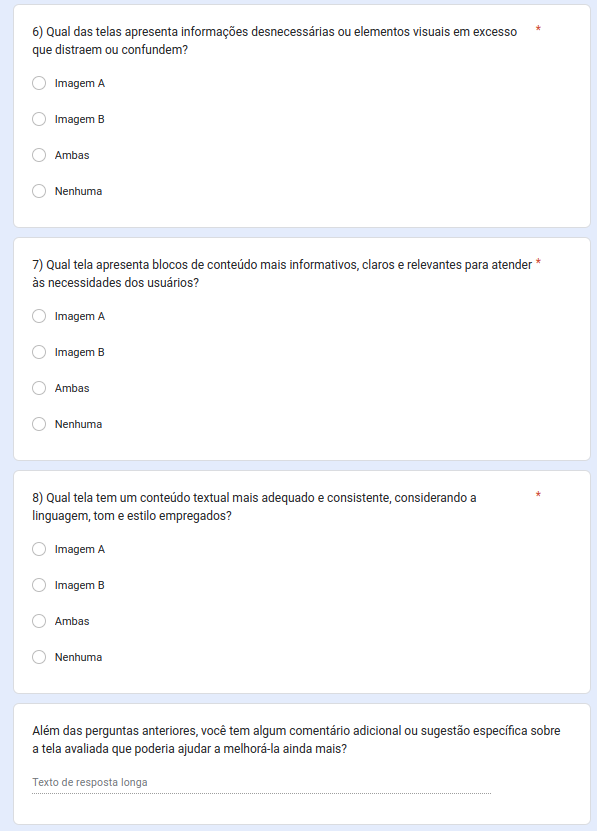
\includegraphics[scale=0.6]{figs/Form/22.png}
	\end{center}
	\caption{\label{AP_PonP04}Formulário de pesquisa, Ponteiro - Parte 4}
\end{figure}
